\renewcommand{\thesection}{Basic Task}

\newcommand{\upa}{\mathlarger{\uparrow}}
\newcommand{\downa}{\mathlarger{\downarrow}}
\newcommand{\lefta}{\mathlarger{\leftarrow}}
\newcommand{\righta}{\mathlarger{\rightarrow}}

\section{Q Learning}

\subsection{Working Environment}

\begin{figure}[h]
	\begin{subfigure}{.49\textwidth}
		\centering
		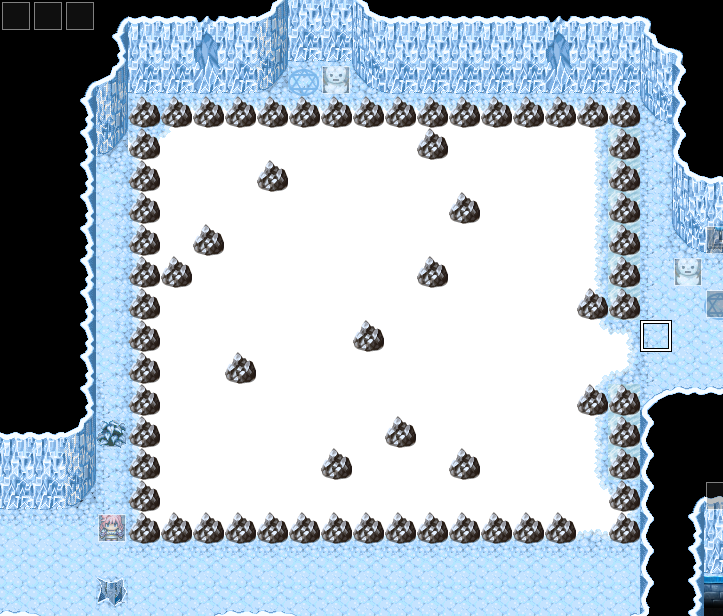
\includegraphics[width=170pt,height=125pt]{snow_original.png}
		\caption{Original puzzle}
	\end{subfigure}
	\begin{subfigure}{.49\textwidth}
		\centering
		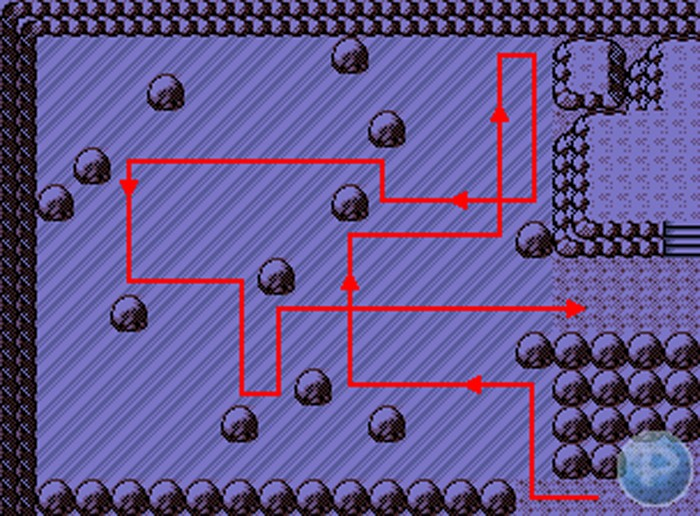
\includegraphics[height=125pt]{snow_2.png}
		\caption{Puzzle solution}
	\end{subfigure}
	\caption{An example of a Pokémon Ice puzzle}
	\label{large_map}
\end{figure}

In this task we present a solver of \emph{Pokémon Ice Puzzles}, a kind of ice puzzle where the player starts at a certain position $s$ and has the objective to reach its objective $e$ in as few steps as possible.

At each turn, the player can do one of four movements: $\{\upa, \downa, \lefta, \righta\}$.
As the environment is ice, when the user walks in any direction is slips on the ice and keeps going on the same direction until hitting a rock or the edge.

The problem statement for the agent is simple: Arrive at the end goal in the least amount of steps possible. The agent would need to know which action constitutes to the next state that leads it closer to the end point.

\newcommand{\coor}[2]{\left\langle #1, #2 \right\rangle}
\newcommand{\yx}{\coor{y}{x}}
\newcommand{\obs}{\mathcal{O}}
\newcommand{\state}{\mathcal{S}}
\newcommand{\reward}{\mathcal{R}}

\subsection{State Transition and Reward Functions}
The state function $\state$, along with the transition and reward functions $\mathcal{T}$ and $\reward$ can be defined as the following, where $\obs_{\yx}$ is true if and only if there is an obstacle on position $\yx$.
\begin{gather*}
	\state = \yx \qquad \mathcal{D} \in \left\{ \upa, \downa, \lefta, \righta \right\} \\
	\begin{aligned}
		&T_{\yx}\left(\upa\right) &= \coor{t + 1}{x} &&&\text{where } \obs_{\coor{t}{x}} \wedge \neg \obs_{\coor{q}{x}} \forall q \in \left(t, y\right) \\
		&T_{\yx}\left(\downa\right) &= \coor{t - 1}{x} &&&\text{where } \obs_{\coor{t}{x}} \wedge \neg \obs_{\coor{q}{x}} \forall q \in \left(y, t\right) \\
		&T_{\yx}\left(\lefta\right) &= \coor{y}{t + 1} &&&\text{where } \obs_{\coor{y}{t}} \wedge \neg \obs_{\coor{y}{q}} \forall q \in \left(t, x\right) \\
		&T_{\yx}\left(\righta\right) &= \coor{y}{t - 1} &&&\text{where } \obs_{\coor{y}{t}} \wedge \neg \obs_{\coor{y}{q}} \forall q \in \left(x, y\right)
	\end{aligned} \\
	\reward(\yx) = \begin{cases}
		100 & \text{if } e = \yx \\
		0 & \text{otherwise}
	\end{cases}
\end{gather*}

In simpler terms, each action the agent makes at a certain point relocates the agent to the last viable open space which is not blocked by the edges of the map or any obstacles. Hence, the states are defined by all the spots that are not occupied by the obstacles or are not edges, while the action space are of the 4 directional functions. It is important to note here that the number of avaiable states are not all squares that are not obstacles or edges, but rather only a select few spaces where the agent can step on when it bumps into the obstacles or edges.

\subsection{Q Function and parameters}

This transition function allows us to define an iterative $Q$ function, which should be used to find the objective $Q^\pi$ function.
\begin{gather*}
	s \in \mathcal{S} \qquad a \in \mathcal{D} \\
	Q^{k + 1}(s, a) = \alpha \cdot \left( \reward( T( a, s ) ) + \gamma \cdot \max{Q^k(s, a)} \right) - Q^k(s, a)
\end{gather*}

The probability next action $a$ is defined depending on the policy used, where $\pi^k(a \mid s)$ represents the probability of choosing action $a$ with state $s$ at point $k$. The variables $\alpha$ and $\gamma$ represent the learning rate and the discount rate respectively, where the former addresses how much the agent learns per step, while the latter defines how much the agent places significance on the current rewards or future rewards.
\begin{gather*}
	\intertext{\textbf{\textepsilon-Greedy Policy}: choose the best policy with probability $\varepsilon$, randomly otherwise.}
	\pi^k(a \mid s) = 
		(1 - \varepsilon) \cdot \frac{1}{\mathcal{D}} + \varepsilon \cdot \begin{cases}
			1 & \text{if } a = \argmax_{a'} (Q^k(s, a')) \\
			0 & \text{otherwise}
		\end{cases} \\
	\intertext{\textbf{Boltzmann Policy}: choose policy using the softmax of the Q-value}
	\pi^k(a \mid s) = \frac{e^{Q^k(s, a)}}{\sum_{a' \in \mathcal{D}}{e^{Q^k(s, a')}}}
\end{gather*}

The epsilon greedy policy starts exploring the environment followed by exploiting, where the agent begins to use the knowledge gained from exploring and derive the best values it sees fit to carry out the actions that gives it the best rewards based on that knowledge. In that sense, the epsilon greedy policy is more deterministic compared to the Boltzmann policy, which also utilises exploration and exploitation, but during exploitation, rather than carrying out the best values it has learnt through exploration, the Boltzmann policy instead chooses an action with probability derived from the equation above. Because of this, the Epsilon-greedy policy is more likely to converge, while the Boltzmann policy is more likely to make more informed actions in cases where two actions in the current time yield marginally different results, leading to more adaptability in more complex environments.

\subsection{Parameter sweep}
\label{param_sweep}
To find the best parameters, we run a parameter sweep on the map in \cref{large_map} for each combination of parameters in \cref{param_sweep_params}; this map is large enough to make it suitable for a parameter sweep.

\begin{table}[h]
	\scriptsize
	\centering
	\begin{tabular}{>{\bfseries}r | l l l l}
		\toprule
		Hyperparameter & \multicolumn{4}{c}{Values} \\
		\midrule
		Policy & \multicolumn{4}{l}{\begin{tabular}{l l}$\varepsilon$-Greedy & Boltzmann\end{tabular}} \\
		$\alpha$ & 0.1 & 0.5 & 0.7 & 0.9 \\
		$\gamma$ & 0.9 & 0.99 && \\
		$\varepsilon$ Decay Rate & 0.75 & 0.9 & 0.99 & \\
		\bottomrule
	\end{tabular}
	\caption{The parameter sweep considered every possible combination of these parameters.}
	\label{param_sweep_params}
\end{table}

Each combination was run 10 times until the Q matrix converged to a precision of $10^{-12}$ and results were averaged.
The final results, which contain the best parameters, can be found in \appendixA{}
Some interesting results can be found in \cref{param_sweep_interesting}.

\begin{table}[h]
	\scriptsize
	\centering
	\begin{tabular}{>{\bfseries}r r l r | r r r r}
		\toprule
		Policy & $\alpha$ & $\gamma$ & $\varepsilon$ Decay &
		E.\ to Conv & Best route & E.\ to Done & E.\ to Best \\
		\midrule
		\rowcolor{YellowGreen}
		\textepsilon{}-Greedy & 0.5  & 0.90  & 0.99 & 139 & 16.00 & 31.80  & 97 \\
		\textepsilon{}-Greedy & 0.9 & 0.90  & 0.90 & 51  & 16.80 & 12.00  & 26 \\
		\midrule
		Boltzmann & 0.2 & 0.90 & 0.75 & 666  & 16.20 &  82.70 &  224 \\
		Boltzmann & 0.9 & 0.90 & 0.99 & 126  & 17.40 &  37.30 &   86 \\
		Boltzmann & 0.7 & 0.90 & 0.75 & 205  & 17.60 &  48.70 &   58 \\
		\bottomrule
	\end{tabular}
	\caption{Some notable results taken from \appendixA{}.}
	\label{param_sweep_interesting}
\end{table}

We can observe the following.
% \begin{itemize}
% 	\item The \textepsilon{}-Greedy policy converges faster and produces a significantly better result.
% 	\item Generally having high $\varepsilon$ Decay represents better results.
% 	\item There is a significant correlation between convergence speed and how good the solutions are.
% \end{itemize}
\subsubsection{Difference in Policies}
The Epsilon-Greedy policy converges faster, as expected from the hypothesis defined above as the Epsilon-Greedy policy is more deterministic as the agent will always take the actions that contain the highest Q-values.  In this sense, the Epsilon-Greedy policy performs better in the ideal scenario that the agent is able to completely learn the environment, meanwhile the Boltzmann policy outperforms the Epsilon-Greedy policy as seen in cases where the agent begins exploiting too early due to low epsilon decay factor, in which case the Boltzmann policy is able to derive a better solution than the Epsilon-Greedy policy as it still considers actions which yield marginally different rewards.

\subsubsection{Difference in epsilon decay factor}
Furthermore, a lower epsilon decay factor generally leads to quicker convergence speeds. This is expected as the epsilon decay factor directly impacts how quickly the agent transitions from exploring to exploiting. 

For most cases, the agent was never able to determine the best route retrospectively (16) as the agent often has already begun exploiting before the agent fully learns the environment provided. This is especially true with epsilon-greedy policies as explained above. 

\subsubsection{Convergence speed vs Solution quality}
Another observation can be made on the tradeoff between the convergence speed and the quality of the solutions, where lower convergence speed allows the agent to learn the environment more and achieve an optimal solution, while a faster convergence speed prompts better training time at the cost of poorer quality solutions.

\subsubsection{Difference in Alphas}
Besides that, a larger alpha directly impacts how much the agent takes the learning in that timestep into account. Excessively large alpha values generally do not perform well as the agent often overestimates the Q-values, leading to the agent to overfit towards certain actions that provide rewards in the first few episodes, causing the agent to be unable to optimize the solution in the environment as the agent already thinks it is doing the best solution. Similarly, excessively low alpha values cause the agent to struggle to find the best solutions locally in a reasonable timeframe. In cases where epsilon decay is low, the agent takes over 400 episodes in both policies to achieve what it believes to be the best result.

\subsection{Analysing this solution}
We choose the parameter combination that converges the fastest between the ones that \emph{always} found the best solution; that's marked in \colorbox{YellowGreen}{green} in table \ref{param_sweep_interesting}

The solution found in \cref{param_sweep} takes on average 139 epochs to converge.
Of those, it takes an average of 31.8 epochs to find a solution, and 97 epochs to find \emph{the best} solution.
Despite taking significantly longer to converge due to its low learning rate, it always finds the optimal solution.

\begin{figure}[H]
	\centering
	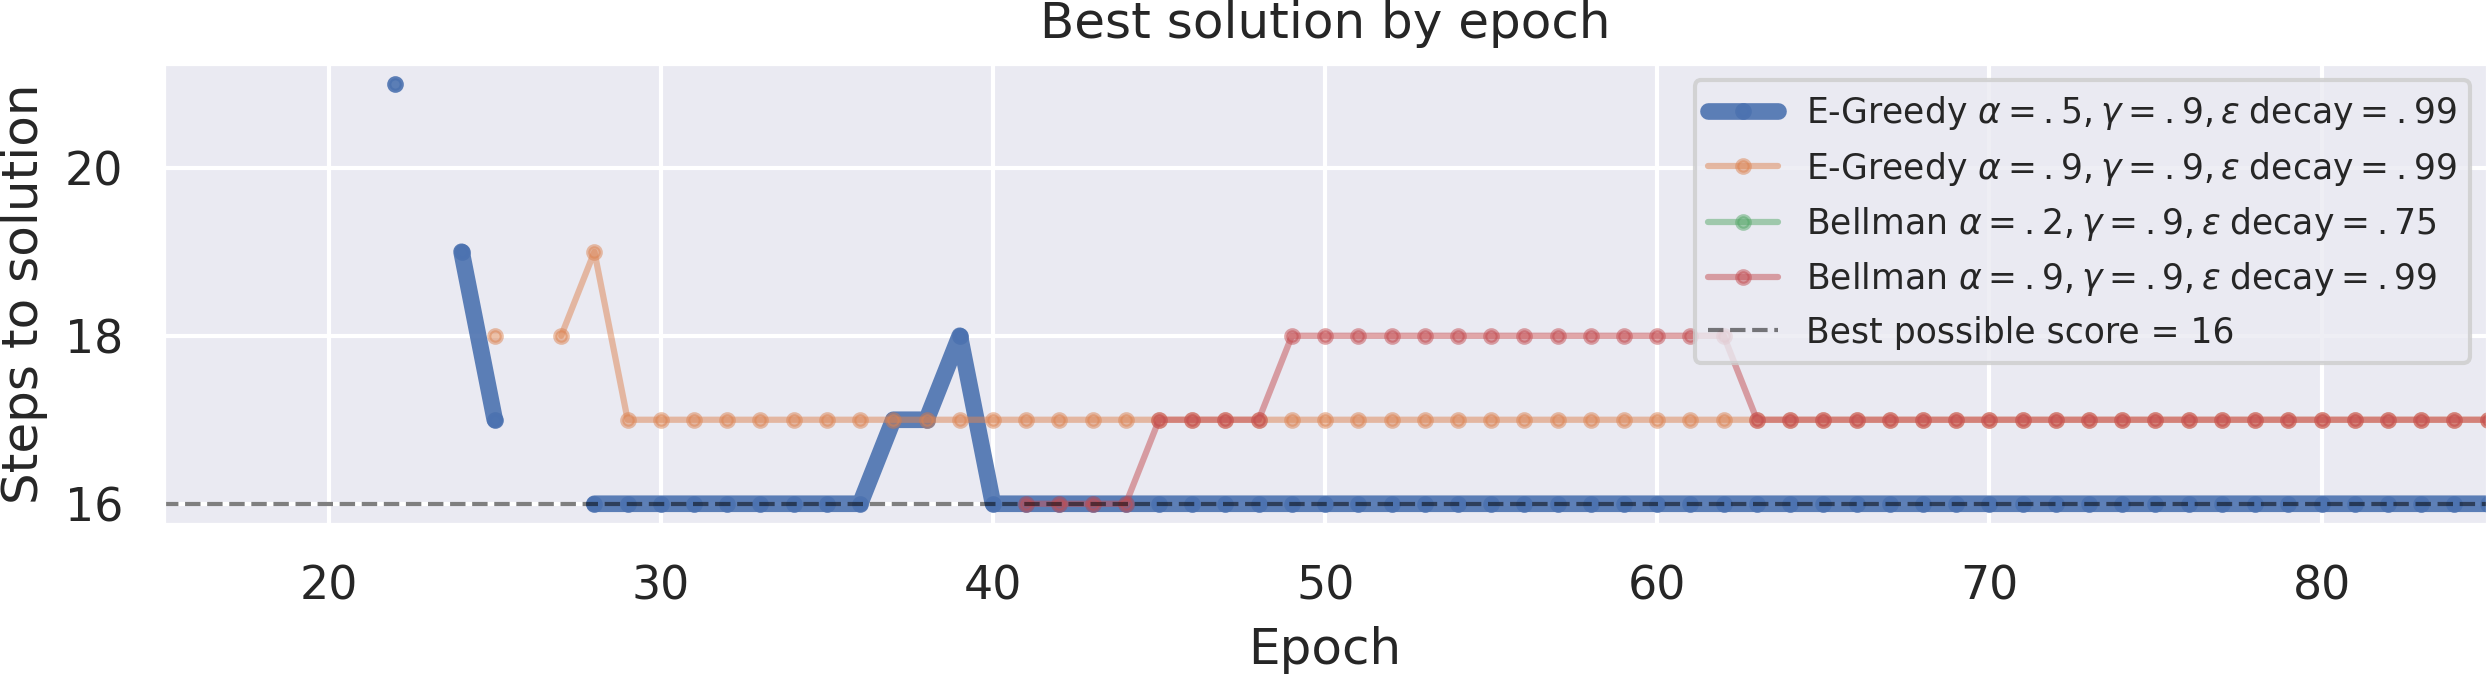
\includegraphics[width=\textwidth]{task1_best_solution_by_epoch.png} \\[1ex]
	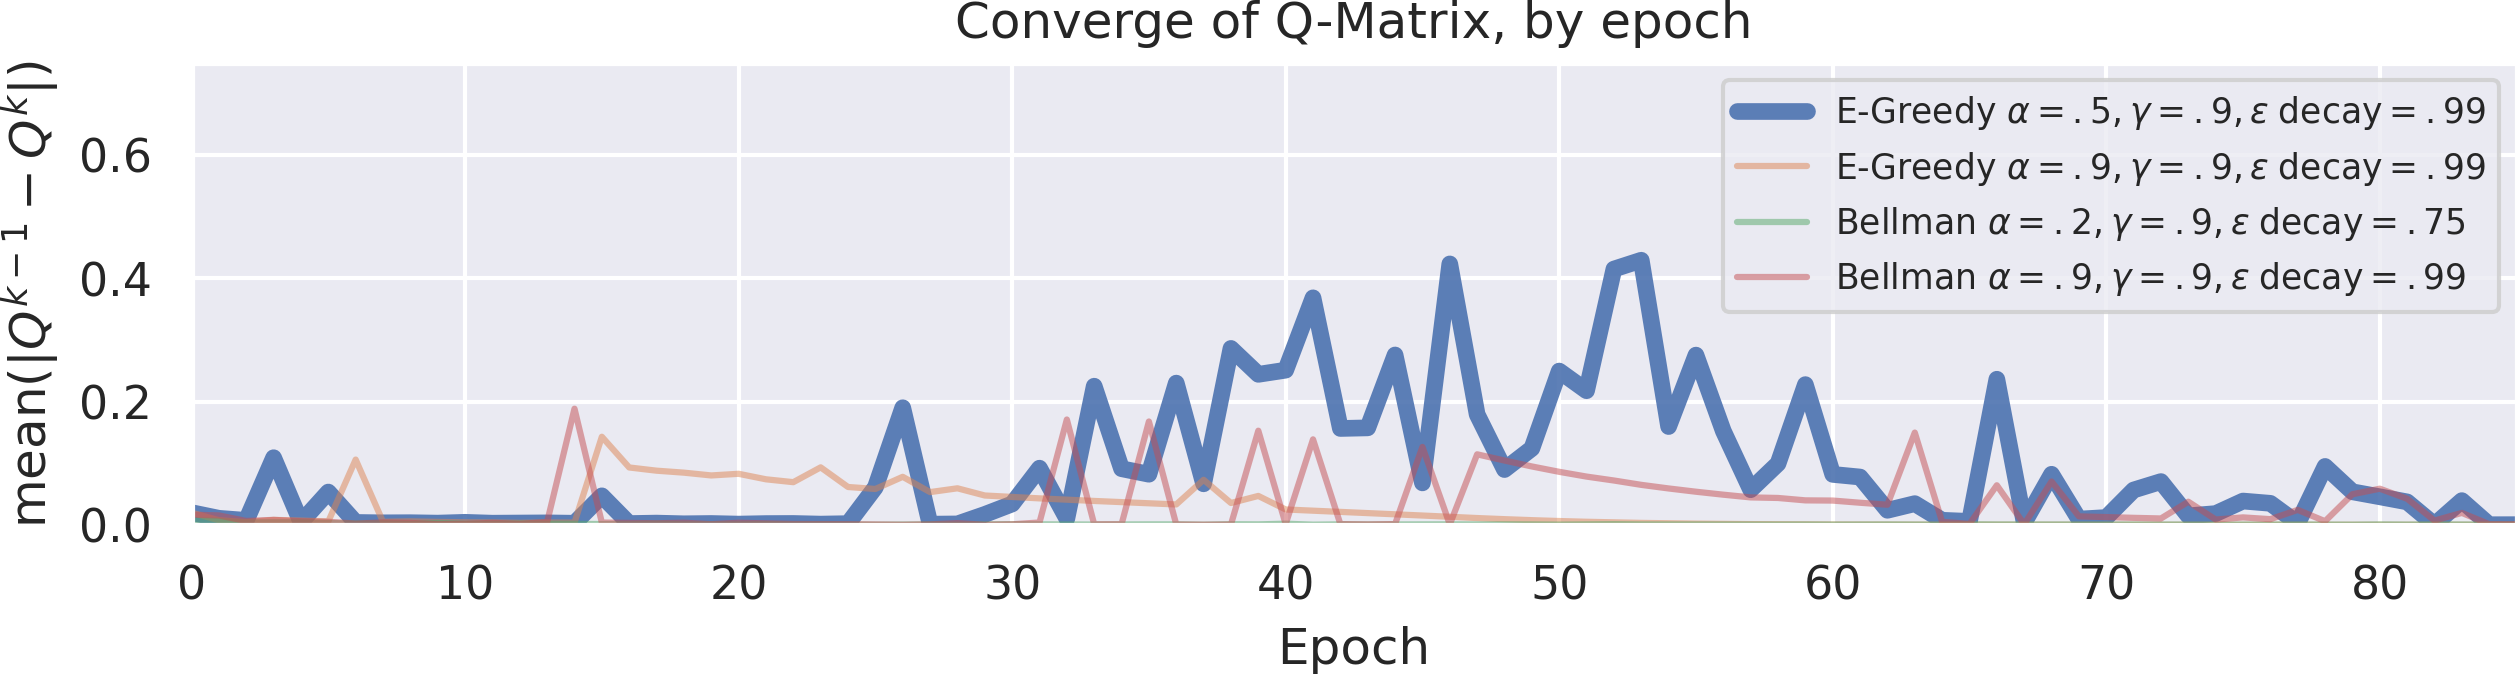
\includegraphics[width=\textwidth]{task1_qmatrix_convergence.png}
	\caption{Best solution found at each epoch and convergence of the Q-matrix of candidate solution and a few others. We can see that the high Epsilon-decay and low learning rate of our chosen solution make it both \emph{a solution} and \emph{the best solution} faster. Additionally, the best solution converges to a much larger mean Q value.}
\end{figure}

\vspace{-13pt}

\renewcommand{\textuparrow}{\ensuremath{\upa{}}}
\renewcommand{\textdownarrow}{\ensuremath{\downa{}}}
\renewcommand{\textleftarrow}{\ensuremath{\lefta{}}}
\renewcommand{\textrightarrow}{\ensuremath{\righta{}}}
\begin{figure}[H]
	\centering
	\begin{subfigure}{.42\textwidth}
		% \resizebox{\textwidth}{!}{\begin{tikzpicture}[every node/.style={anchor=center}]
	\matrix (table) [
		matrix of nodes,
		nodes={draw, minimum height=20pt, minimum width=20pt, anchor=center, line width=.1pt},
		nodes in empty cells,
		execute at begin node = $,
		execute at end node = $,
		column 1/.style={nodes={fill=gray!30, execute at begin node=$, execute at end node=$}},
		row 1/.style={nodes={fill=gray!30, execute at begin node=$, execute at end node=$}}
	]{
   & 0 & 1 & 2 & 3 & 4 & 5 & 6 & 7 & 8 & 9 & 10 & 11 & 12 \\
 0 & → & ↓ & ← & ← & → & ↓ & ↓ & ↓ & |[fill=Gray]| x & ↓ & → & ← & ← \\
 1 & → & ↑ & ← & |[fill=Gray]| x & → & ← & ← & → & ← & ← & → & ← & ↓ \\
 2 & ↓ & → & → & → & ← & ↑ & ↓ & ↑ & ↑ & |[fill=Gray]| x & ↓ & → & ← \\
 3 & ↑ & |[fill=Gray]| x & ↓ & ↓ & ↓ & → & ← & → & → & ← & → & ↑ & ← \\
 4 & |[fill=Gray]| x & → & ↑ & → & ← & → & → & ← & |[fill=Gray]| x & ↑ & ← & ← & ← \\
 5 & → & ← & ↓ & ↓ & ↑ & ← & → & ↓ & → & → & ↑ & ↑ & |[fill=Gray]| x \\
 6 & → & ← & → & ↑ & ← & ↑ & |[fill=Gray]| x & ↑ & ← & ↓ & ↑ & ↑ & ↓ \\
 7 & ↓ & ↑ & |[fill=Gray]| x & ↓ & → & ↓ & → & ↓ & ← & ← & ↑ & → & |[fill=Yellow]| \checkmark{} \\
 8 & → & ← & → & ↑ & ↑ & → & → & ↑ & → & ← & ← & ← & |[fill=Gray]| x \\
 9 & → & ↑ & ← & → & ↓ & ← & ↑ & |[fill=Gray]| x & ↑ & ↑ & ← & ↑ & ← \\
10 & → & ↑ & ↑ & ↑ & ↓ & |[fill=Gray]| x & ↓ & ↓ & ← & |[fill=Gray]| x & ↑ & ↓ & ← \\
11 & ↑ & ← & → & → & ↑ & → & ↑ & ↑ & → & → & ↑ & ↑ & ← \\
12 & |[fill=Gray]| x & |[fill=Gray]| x & |[fill=Gray]| x & |[fill=Gray]| x & |[fill=Gray]| x & |[fill=Gray]| x & |[fill=Gray]| x & |[fill=Gray]| x & |[fill=Gray]| x & |[fill=Gray]| x & |[fill=Gray]| x & |[fill=Gray]| x & |[fill=LimeGreen]|↑ \\
	};

	\foreach \row in {2,...,14} {
		\foreach \col in {2,...,14} {
			\pgfmathtruncatemacro{\rown}{\row - 2} % Adjust row number
			\pgfmathtruncatemacro{\coln}{\col - 2} % Adjust column number
			\node (c-\rown-\coln) at (table-\row-\col) {};

			\edef\cellname{c-\rown-\coln}
			\foreach \dir/\dx/\dy in {u/0/6pt, d/0/-6pt, l/-6pt/0, r/6pt/0, 
									  ul/-6pt/6pt, ur/6pt/6pt, 
									  dl/-6pt/-6pt, dr/6pt/-6pt} {
				\path (\cellname.center) ++(\dx, \dy) node (\cellname\dir) {};
			}
		}
	}
	\node[fit=(table-1-1)(table-14-14), draw, very thick, inner sep=0pt] {};

\draw [->, ultra thick]
(c-12-12dr.center) -- (c-9-12ur.center) -- (c-9-8ul.center) -- (c-5-8ul.center) -- (c-5-11ur.center) -- (c-0-11ur.center) -- (c-0-9ul.center) -- (c-1-9dl.center) -- (c-1-4dl.center) -- (c-1-4ul.center) -- (c-1-12ur.center) -- (c-4-12dr.center) -- (c-4-9dl.center) -- (c-3-9ul.center) -- (c-3-2ul.center) -- (c-6-2dl.center) -- (c-6-5dr.center) -- (c-0-5ur.center) -- (c-0-5ul.center) -- (c-9-5dl.center) -- (c-9-0dl.center) -- (c-9-0ul.center) -- (c-9-6ur.center) -- (c-7-6ur.center) -- (c-7-12ur.center);


\end{tikzpicture}

}
		\caption{After 23 epochs, with a path of length 24.}
	\end{subfigure}
	\begin{subfigure}{.42\textwidth}
		% \resizebox{\textwidth}{!}{\begin{tikzpicture}[every node/.style={anchor=center}]
	\matrix (table) [
		matrix of nodes,
		nodes={draw, minimum height=20pt, minimum width=20pt, anchor=center, line width=.1pt},
		nodes in empty cells,
		execute at begin node = $,
		execute at end node = $,
		column 1/.style={nodes={fill=gray!30, execute at begin node=$, execute at end node=$}},
		row 1/.style={nodes={fill=gray!30, execute at begin node=$, execute at end node=$}}
	]{
		& 0 & 1 & 2 & 3 & 4 & 5 & 6 & 7 & 8 & 9 & 10 & 11 & 12 \\
		0 & → & ↓ & ↓ & → & ↓ & ↓ & ↓ & ↓ & |[fill=Gray]| x & → & → & → & ↓ \\
		1 & → & ↓ & ↑ & |[fill=Gray]| x & → & → & ↓ & ↑ & ↓ & → & ← & ↓ & ↓ \\
		2 & ↓ & ← & ↑ & ← & → & ↓ & ← & → & ↑ & |[fill=Gray]| x & → & → & ↓ \\
		3 & ↑ & |[fill=Gray]| x & ↓ & → & → & ↓ & ← & ← & → & ← & ← & ↑ & ← \\
		4 & |[fill=Gray]| x & ↓ & ↓ & ↓ & → & ← & ← & ← & |[fill=Gray]| x & ↑ & ↓ & ↓ & ← \\
		5 & → & ↓ & ← & ↓ & → & → & → & ← & → & ↓ & ↓ & ↑ & |[fill=Gray]| x \\
		6 & → & ← & → & → & ← & ↓ & |[fill=Gray]| x & → & → & → & ↑ & ↑ & ↓ \\
		7 & ↓ & ← & |[fill=Gray]| x & → & ← & → & → & → & ↑ & ↑ & → & → & |[fill=Yellow]|\checkmark{} \\
		8 & → & ← & ↓ & ↓ & ← & ↑ & → & → & ↓ & ↓ & ↑ & ↓ & |[fill=Gray]| x \\
		9 & → & ↓ & ↓ & → & ↑ & → & ↑ & |[fill=Gray]| x & ↑ & ↑ & ← & ↑ & ← \\
		10 & ↓ & → & ↓ & ↑ & ↓ & |[fill=Gray]| x & ↓ & ↓ & ↑ & |[fill=Gray]| x & ↓ & ← & ↓ \\
		11 & ↑ & → & → & ← & ↑ & ← & ↑ & ← & ↑ & ← & ↑ & ↑ & ↑ \\
		12 & |[fill=Gray]| x & |[fill=Gray]| x & |[fill=Gray]| x & |[fill=Gray]| x & |[fill=Gray]| x & |[fill=Gray]| x & |[fill=Gray]| x & |[fill=Gray]| x & |[fill=Gray]| x & |[fill=Gray]| x & |[fill=Gray]| x & |[fill=Gray]| x & |[fill=Green]|↑ \\
	};

	\foreach \row in {2,...,14} {
		\foreach \col in {2,...,14} {
			\pgfmathtruncatemacro{\rown}{\row - 2} % Adjust row number
			\pgfmathtruncatemacro{\coln}{\col - 2} % Adjust column number
			\node (c\rown\coln) at (table-\row-\col) {};

			\edef\cellname{c\rown\coln}
			\foreach \dir/\dx/\dy in {u/0/6pt, d/0/-6pt, l/-6pt/0, r/6pt/0, 
									  ul/-6pt/6pt, ur/6pt/6pt, 
									  dl/-6pt/-6pt, dr/6pt/-6pt} {
				\path (\cellname.center) ++(\dx, \dy) node (\cellname\dir) {};
			}
		}
	}
	\node[fit=(table-1-1)(table-14-14), draw, very thick, inner sep=0pt] {};

	\draw [->, ultra thick]
		(c1212r.center) -- (c912ur.center) -- (c98ul.center) -- (c58ul.center) --
		(c511ur.center) -- (c011ur.center) -- (c012ur.center) -- (c412dr.center) --
		(c49dl.center) -- (c39ul.center) -- (c32ul.center) -- (c62dl.center) --
		(c65dr.center) -- (c95dr.center) -- (c96dr.center) --
		(c76ur.center) -- (c712u.center);

\end{tikzpicture}

}
		\caption{After 100 epochs, with an ideal path of length 16.}
	\end{subfigure}
	\caption{Best action according to each state of the Q-matrix after different amounts of epochs.}
\end{figure}
